\documentclass[12pt,openright,twoside,french]{book}

\input philippe2013
\input philippe2013_activites
\pagestyle{empty}


\begin{document}

\TitreActivite{xi.1}{Dérivation \\ Tangente à une courbe}

Le bénéfice d'une entreprise est calculé, en euros, par la formule suivante : \[B(x) = 10x - 0,01 x^2\] où $x$ représente le nombre de produits vendus tel que $0 \leq x \leq \np{1000}$.\par
La courbe représentative $\calig C_B$ est tracée ci-dessous :

\begin{center}
    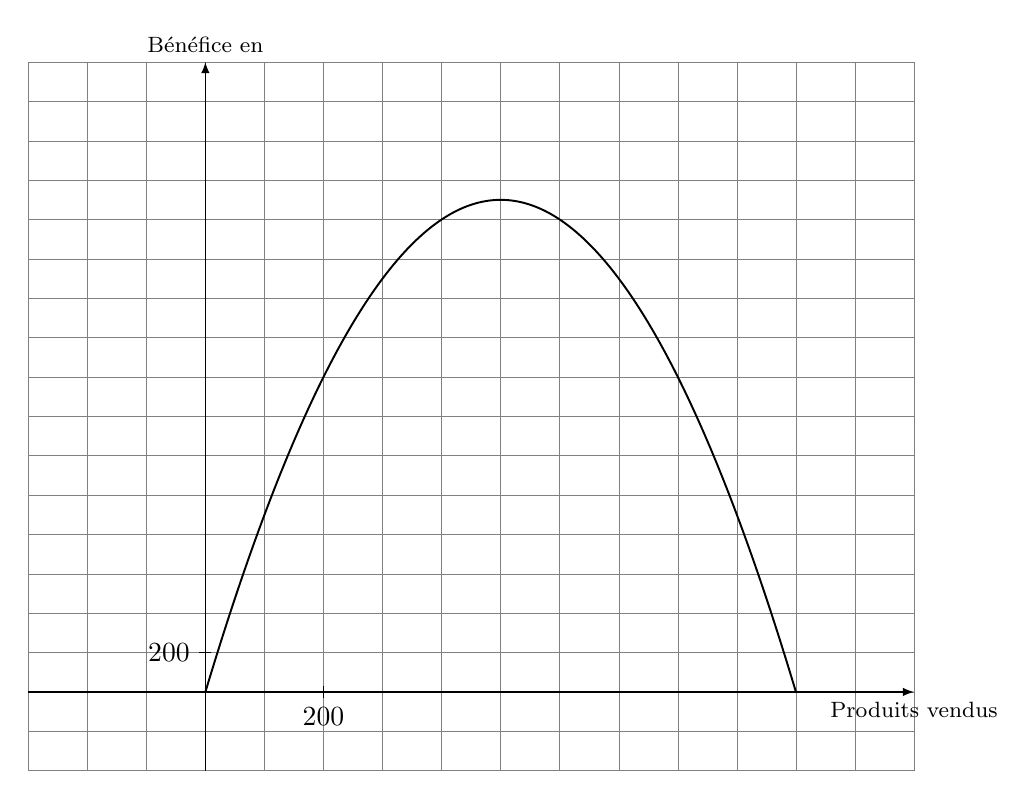
\begin{tikzpicture}[>=latex,y=0.25cm,x=0.75cm]
        \draw[help lines] (-3,-4) grid[xstep=1,ystep=2] (12,32);
        \draw[->] (-3,0) -- (12,0) node[below] {\footnotesize Produits vendus};
        \draw[->] (0,-4) -- (0,32) node[above] {\footnotesize Bénéfice en \EUR{}};
        \draw[line width=0.7pt] plot[domain=0:10,samples=200] (\x,{-(\x)^2 + 10*\x});
        \draw (2,0.3)--(2,-0.3) node[below] {$200$};
        \draw (0.1,2)--(-0.1,2) node[left] {$200$};
    \end{tikzpicture}
\end{center}

\begin{enumerate}
    \item Compléter le tableau de valeur suivant :
    \begin{center}
    \renewcommand\arraystretch{2}
        \begin{tabularx}{0.75\linewidth}{|*{7}{>{\centering\arraybackslash} X|}}
        \hline
            $x$ & $200$ & $400$ & $500$ & $600$ & $800$ & $1000$ \\
        \hline
            $R(x)$ & & & & & & \\
        \hline
        \end{tabularx}
    \end{center}

    \item \textbf{Calculer} le nombre de produit à vendre pour obtenir un bénéfice maximal. Déterminer ce bénéfice par le calcul.
    \item Calculer la variation du bénéfice entre $200$ produits vendus et $400$ produits vendus ?
    \item En déduire la variation moyenne par produit du bénéfice dans ces conditions.
    \item Tracer la droite passant par les points $A(200 \pv \np{1600})$ et $B(400 \pv \np{2400})$. Quel est le c{\oe}fficient directeur de cette droite ?
    \item Calculer la variation du bénéfice entre $500$ produits vendus et $800$ produits vendus puis le bénéfice moyen par produit.
    \item On veut connaître la variation moyenne du bénéfice pour une quantité très proche de $200$ produits vendus. Quelle solution graphique peut-on envisager ?
\end{enumerate}
\end{document} 